% !TeX spellcheck = de_DE
\section{NeuroEvolution of Augmenting Topologies}
\label{sec:neat}
Der in dieser Arbeit verwendete Algorithmus heißt \ac{NEAT}, welcher im Jahr 2002 von \citeauthor{stanley2002evolving} vorgestellt wurde. Bei der Veröffentlichung hat \ac{NEAT} für die meisten Optimierungsprobleme im Vergleich zu anderen Verfahren schneller Lösungen gefunden, obwohl es neben den Gewichten des \ac{KNN} auch die Struktur optimiert \cite{stanley2002evolving}. Somit gehört der Algorithmus zur Gruppe der \ac{TWEANN} Algorithmen. Heute gilt \ac{NEAT} immer noch als einer der bekanntesten Vertretern der neuroevolutionären Algorithmen und dient als Basis für viele Erweiterungen wie zum Beispiel HyperNEAT, cgNEAT, ... \\
% TODO Add NEAT Sources
Für die guten Ergebnisse sind drei Eigenschaften besonders relevant \cite{stanley2002evolving}:
\begin{enumerate}
	\item Erfolgreiche Reproduktion trotz verschiedener Strukturen
	\item Schützen von neuen Innovationen durch verschiedene Spezies
	\item Wachsen einer minimalen Struktur
\end{enumerate}
In diesem Kapitel wird die grundsätzliche Funktionsweise von \ac{NEAT} erläutert, wie sie in der originalen Publikation vorgestellt ist. Wenn nicht anderweitig gekennzeichnet, beziehen sich alle Informationen aus diesem Kapitel auf Quelle \cite{stanley2002evolving}. Für eine bessere Lesbarkeit wird in diesem Kapitel auf weitere Zitierungen verzichtet.
\subsection{Kodierung}
\label{subsec:neat_encoding} % TODO ABBILDUNG
\begin{figure}[!h]
	\centering
	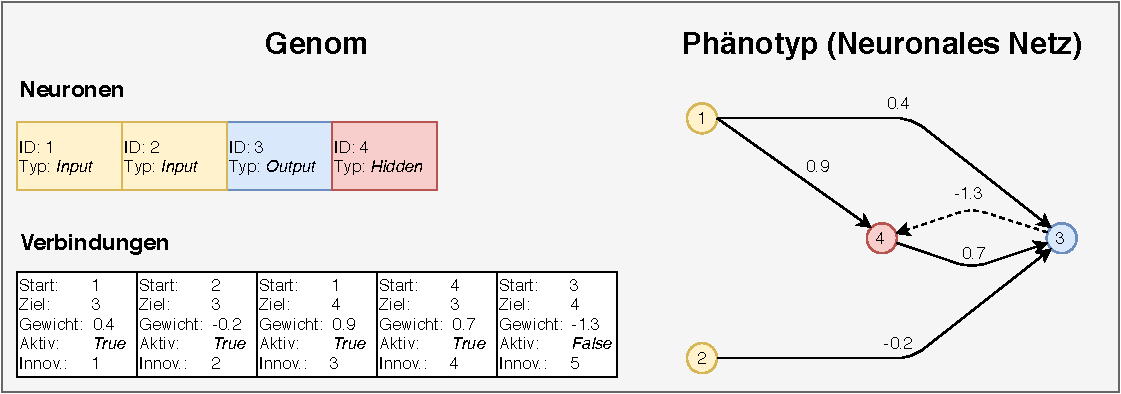
\includegraphics[width=1\textwidth]{./img/neat_genome_encoding.pdf} 
	\caption{Schematische Darstellung von einem Genom mit dazugehörigem Phänotyp}
	\label{fig:neat_encoding}
\end{figure}
\ac{NEAT} verwendet ein direktes Kodierungsverfahren. Ein Genom enthält, wie in Abbildung (TODO ABBILDUNG) beispielhaft dargestellt, je eine Liste für Neuronen und Verbindungen. Ein Neuron wird durch eine ID identifiziert und enthält den Typ (\emph{Input}, \emph{Output}, \emph{Hidden}). Eine Verbindung enthält das Start- und Zielneuron, das dazugehörige Gewicht, ein Aktivierungsbit sowie eine Innovationsnummer. Das Aktivierungsbit gibt an, ob die Verbindung im Phänotyp, in diesem Fall dem neuronalen Netz enthalten, ist. Auf die Funktionsweise und Bedeutung der Innnovationsnummer wird später genauer eingegangen.
\subsection{Mutation}
\label{subsec:neat_mutation}
Ein Genom kann auf verschiedene Arten mutieren, welche entweder die Struktur des \ac{KNN} oder die Gewichte der Verbindungen beeinflussen. Die Mutation der Gewichte ist ähnlich zu anderen neuroevolutionären Algorithmen. Für jedes Gewicht besteht eine Wahrscheinlichkeit zur Mutation. In diesem Fall wird das Gewicht entweder leicht abgeändert oder ein neuer zufälliger Wert gewählt.\\ % TODO ABBILDUNG
\begin{figure}[!h]
	\centering
	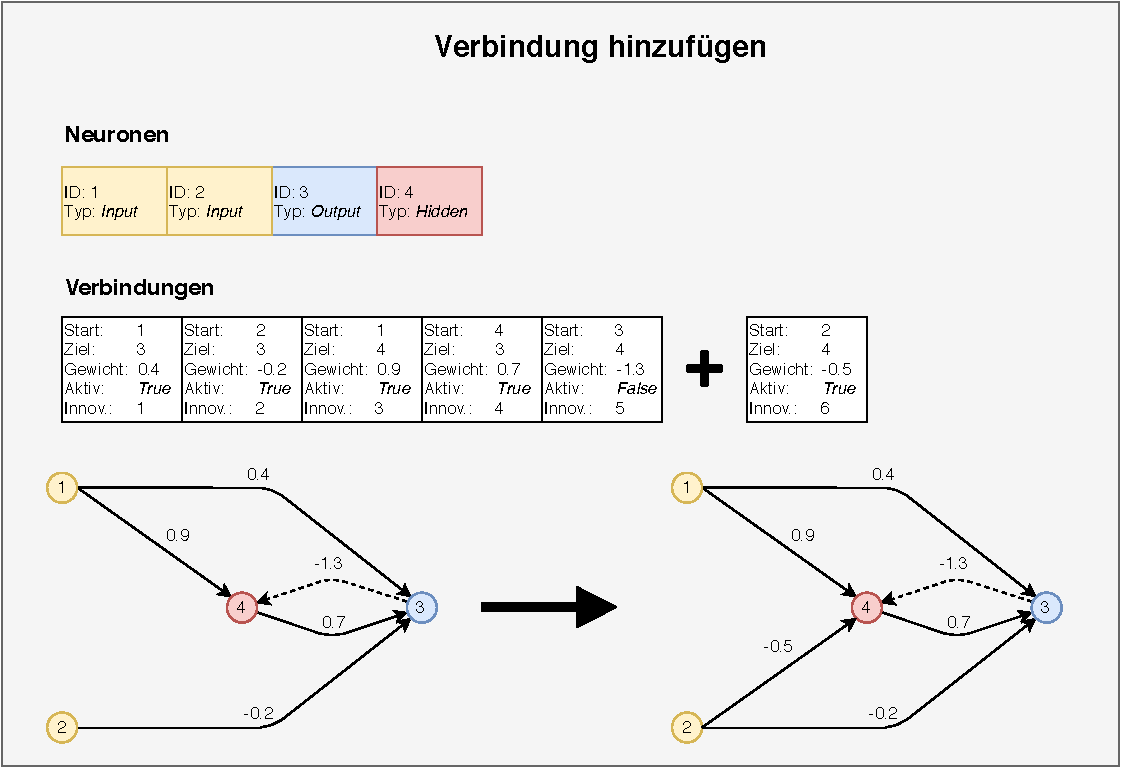
\includegraphics[width=1\textwidth]{./img/neat-AddConnectionMutation.pdf} 
	\caption{Schematische Darstellung von einem Genom mit dazugehörigem Phänotyp}
	\label{fig:neat_add_connectin_mutation}
\end{figure}
Strukturelle Mutationen können in zwei verschiedenen Arten auftreten. Bei der ersten wird eine einzelne neue Verbindung dem Genom hinzugefügt. Bei der Auswahl des Start- und Zielneurons ist zu beachten, dass diese nicht bereits über eine solche Verbindung verfügen. Das Gewicht für die neue Verbindung wird zufällig gewählt und das Aktivierungsbit auf \emph{True} gesetzt. Ein Beispiel für diese Mutation ist in Abbildung (TODO ABBILDUNG) dargestellt. Bei der zweiten Art der strukturellen Mutation wird ein neues Neuron das \ac{KNN} eingefügt. Hierzu wird zu Beginn eine aktive Verbindung $con_{ij} $ zufällig ausgewählt, welche von Neuron $i$ zu Neuron $j$ führt. Anschließend wird ein neues Neuron $x$ zwischen den Neuronen $i$ und $j$ platziert und zwei weitere Verbindungen werden hinzugefügt. Die erste Verbindung $con_{ix}$ führt vom alten Startneuron $i$ zum neu hinzugefügtem und erhält das Gewicht $1$. Die zweite Verbindung $con_{xj}$ beginnt bei dem neuen Neuron und endet im dem alten Zielneuron $j$ und erhält dasselbe Gewicht wie die Verbindung $con_{ij}$. Zuletzt wird die ausgewählte Verbindung $con_{ij}$ deaktiviert, indem das Aktivierungsbit auf $False$ gesetzt wird. Diese Art der Mutation reduziert den initialen Effekt des neuen Neurons. So kann es direkt vom \ac{KNN} verwendet werden, ohne dass die Verbindungsgewichte stark optimiert werden müssen.
\begin{figure}[!h]
	\centering
	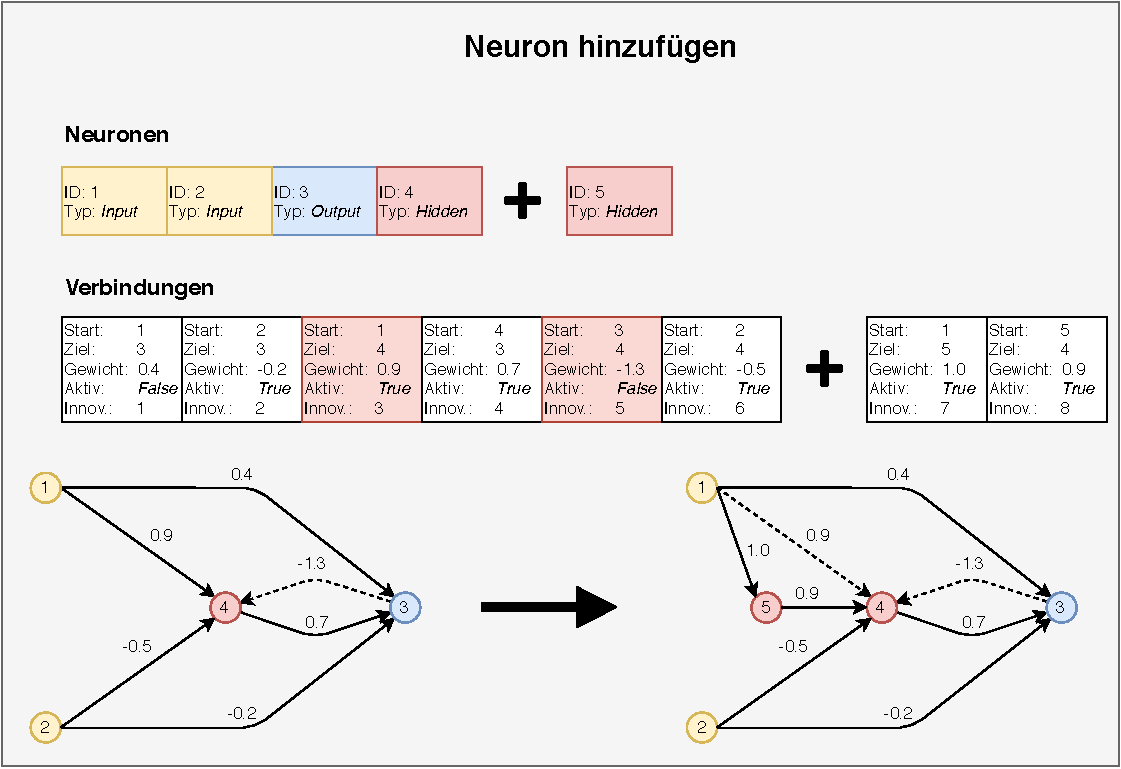
\includegraphics[width=1\textwidth]{./img/neat-AddNodeMutation.pdf} 
	\caption{Schematische Darstellung von einem Genom mit dazugehörigem Phänotyp}
	\label{fig:neat_add_node_mutation}
\end{figure}
\subsection{Reproduktion}
\label{subsec:neat_reproduction}
Das Ergebnis der in Kapitel \ref{subsec:neat_mutation} vorgestellten Mutationen ist eine Population mit verschieden Genomen, welche unterschiedliche Gewichte und Strukturen haben können. Dies ist die schwierigste Form des in Kapitel \ref{subsec:competing_convention_problem} vorgestellten \emph{competing convention} Problems und macht das Erstellen von Nachkommen besonders schwierig.\\
\ac{NEAT} löst dieses Problem, indem es den historischen Ursprung von jeder strukturellen Mutation überwacht. Haben zwei Verbindungen denselben Ursprung, haben sie in der Vergangenheit dieselbe Struktur repräsentiert, auch wenn sie inzwischen unterschiedliche Gewichte haben. Zu diesem Zweck besitzt jede Verbindungen die im Kapitel \ref{subsec:neat_encoding} erwähnte Innovationsnummer. Jedes Mal, wenn eine neue Verbindung entsteht, wird ein globaler Zähler inkrementiert und der Wert als Innovationsnummer der Verbindung verwendet. Abbildung (TODO ABBOLDUNG) zeigt die Zuweisung beispielhaft. Die erste Mutation, welche nur eine neue Verbindung herstellt, hat die Innovatiosnummer X zugewiesen bekommen. Wenn im Folgenden ein neues Neuron mit zwei weiteren Verbindungen hinzugefügt wird, erhalten diese die Nummern Y und Z. Werden Verbindungen von einem Genom in der Reproduktiosnphase für die Nachkommen ausgewählt, wird auch die Innovationsnummer übertragen. Somit ist auch bei den nachfolgenden Generationen ersichtlich, was der historische Ursprung einer Verbindung ist. Tritt durch Zufall dieselbe Mutation in einer Generation mehrfach auf, erhalten die neuen Verbindungen dieselben Innovationsnummern. Hierfür müssen alle aufgetretenen Mutation einer Generation zwischengespeichert werden. \\
Die Innovationsnummern können nicht nur ressourcensparend implementiert werden, sie machen auch das Erzeugen von Nachkommen in der Reproduktionsphase bedeutend einfacher, da beim Kreuzen von zwei Elternteilen keine aufwendige Strukturanalyse erforderlich ist. Abbildung (TODO ABBILDUNG) zeigt beispielhaft, wie ein Nachkommen aus zwei Elterngenomen $X$ und $Y$ entsteht. Die sogenannten \emph{maching genes} sind Verbindungen, deren Innovationsnummern in beiden Elterngenomen vorkommen. Beim Erstellen der Nachkommen wird für jede Verbindung in den \emph{matching genes} zufällig entschieden, aus welchem Elternteil diese übernommen wird. Die sogenannten \emph{disjoint genes} und \emph{excess genes} sind Verbindungen, die nur in einem Elternteil vorkommen. Zu den \emph{disjoint genes} gehören die Verbindungen, deren Innovationsnummer kleiner als die größte Innovationsnummer des zweiten Elterngenoms ist. Die \emph{excess genes} sind Verbindungen, deren Innovationsnummer größer als die höchste Innovationsnummer im anderen Elternteil ist. Beim Erzeugen von Nachkommen werden nur die \emph{excess genes} und \emph{disjoint genes} von dem Elternteil übernommen, welches den höheren Fitnesswert erzielt hat. Haben beide Elternteile den selben Wert, werden die Verbindungen von beiden übernommen.
Bei dieser Implementierung wird angenommen, dass der Schwellwert der Neuronen, wie in Kapitel (TODO KAPITE) erläutert, durch eine Verbindung zu einem Bias-Neuron ausgedrückt wird. Dadurch enthalten die Neuronen keine spezifischen Informationen, die sich zwischen den Elterngenomen unterscheiden. Die Nachkommen übernehmen deshalb immer die Neuronen des Elternteils mit dem größeren Fitnesswert.
\subsection{Spezies}
\label{subsec:neat_species}
Die vorgestellten Arten der Mutation und die erfolgreiche Reproduktion ermöglichen es \ac{NEAT}, eine Population mit vielen verschiedenen Strukturen zu entwickeln. Dennoch reichen diese Faktoren nicht aus, da in der Praxis neue strukturelle Innovationen nur eine geringe Chance haben, langfristig integriert zu werden und es wahrscheinlicher ist, dass sie nach wenigen Generation aussterben. Die Gründe hierfür sind, dass kleinere \ac{KNN} schneller optimiert werden können als große und dass das Hinzufügen von neuen Neuronen und Verbindungen den Fitnesswert meistens initial senkt, auch wenn die neuen Strukturen für das erfolgreiche Lösen des Optimierungsproblems notwendig sind. Die Folge ist, dass die kleinen Genome anfänglich bessere Fitnesswerte erzielen, die größeren Genome nicht für die Reproduktion ausgewählt werden wodurch die strukturellen Innovationen wieder verloren gehen.
\\\\
Das Problem wird von \ac{NEAT} durch das Einführen von verschiedenen Spezies gelöst. Das Ziel ist, Genome, die sich strukturell ähnlich sind in einer Spezies zu gruppieren. Bei der Auswahl der Elterngenome für die Nachkommen muss ein Genom nicht mehr mit der ganzen Population konkurrieren, sondern nur noch mit den anderen Genomen der eigenen Spezies. Somit sind neue Innovationen erst einmal in ihrer Spezies vor dem Aussterben geschützt und können mit der Zeit optimiert werden. Für die Implementierung eines solchen Verfahrens wird eine Funktion benötigt, die messen kann, wie ähnlich oder unterschiedlich zwei Genome sind. Auch hier kann wie bei der Rekombination auf eine aufwendige Strukturanalyse verzichtet werden, da dies mit den bereits bekannten Innovationsnummern umsetzbar ist. Je mehr \emph{excess genes} und \emph{disjoint genes} zwei Genome besitzen, desto weniger evolutionäre Geschichte teilen sie und sind somit unterschiedlicher. Auch der Gewichtsunterschied ist ein wichtiger Faktor, wie in Kapitel \ref{subsec:competing_convention_problem} dargestellt. Die von \ac{NEAT} verwendete Formel, um die Kompatibilität $\delta$ zwischen zwei Genomen zu berechnen, ist im Folgenden abgebildet:
$$\delta=\frac{c_1E}{N}+\frac{c_2D}{N}+c_3 \cdot \overline{W}$$
Die Variablen $E$ und $D$ ergeben sich aus der Anzahl an \emph{excess genes} und \emph{disjoint genes}. $\overline{W}$ ist die durchschnittliche Gewichtsdifferenz der \emph{matching genes}. Die Faktoren $c_1$, $c_2$ und $c_3$ ermöglichen es die Wichtigkeit der einzelnen Komponenten je nach Optimierungsproblem zu justieren. $N$ steht für die Anzahl der Verbindungen im größeren Genom und normalisiert die Anzahl der \emph{excess genes} und \emph{disjoint genes}. Somit ist der Effekt auf den Kompatibilitätswert $\delta$ bei einer neuen Verbindung in großen Genomen gering und in kleinen sehr groß. Je nach Konfiguration kann für kleine Genome $N=1$ gelten.
\\\\
Die Zuordnung von neu erstellten Genomen zu einer Spezies erfolgt nach der Reproduktions- und Mutationsphase. Hierfür wird eine geordnete Liste mit allen verfügbaren Spezies benötigt. Jede Spezies wird durch ein Genom repräsentiert, welches in der vorherigen Generation ein Mitglied von dieser war. Bei der Zuordnung von einem Genom wird über die Liste der Spezies iteriert und zu jedem Repräsentanten der Kompatibilitätswert $\delta$ gebildet. Ist $\delta \leq \delta_t$, wobei $\delta_t$ ein konfigurierbarer Schwellwert ist, wird das Genom der Spezies zugeordnet und die Suche abgebrochen. Ist das Genom zu keiner Spezies kompatibel, wird eine neue erstellt und das Genom als Repräsentant gesetzt.
\\\\
Zum erhalten von verschiedenen Strukturen muss verhindert werden, dass eine Spezies zu groß wird und die restlichen verdrängt auch wenn viele der Mitglieder gute Fitnesswerte erzielen. Zusätzlich müssen vorallem neue Spezies geschützt werden. Diese haben initial wenige Mitglieder und somit eine geringere Chance als Elterngenome ausgewählt zu werden. Zum Lösen dieses Problems verwendet \ac{NEAT} sogenanntes \emph{explicit fitness sharing}, welches 1987 von \citeauthor{goldberg1987genetic} in ihrer Arbeit \cite{goldberg1987genetic} vorgestellt wurde. Jede Spezies bekommt bei der Reproduktion eine Anzahl an Nachkommen zugewiesen, welche proportional zu der Fitness $f_{s}$ der Spezies ist. Diese ergibt sich aus der Summe aller angepassten Fitnesswerte $f'$ der Mitglieder. Der angepasste Fitnesswert $f'$ eines Genoms wird berechnet indem die erreichte Fitness $f$ durch die Anzahl an Mitgliedern in der Spezies geteilt wird. Das Ziel dieser Maßnahme ist, dass große Spezies im Vergleich zu kleinen benachteiligt werden und kleine erfolgreiche Spezies entsprechend viele Nachkommen zugewiesen bekommen. Ein Beispiel hierfür ist in Abbildung xy (TODO ABBILDUNG) dargestellt. Obwohl die zweite Spezies bedeutend weniger, aber dafür gute Genome besitzt, werden ihr mehr Nachkommen zugewiesen. Würden die Anzahl von Nachkommen einer Spezies proportional zu der Summe der erreichten Fitnesswerte vergeben, hätte die kleinere Spezies weniger zugewiesen bekommen. 
\\\\
Ist der Fitnesswert $f_s$ von jeder Spezies berechnet und die Nachkommen proportional zugeteilt beginnt die Reproduktion. Die Elterngenome werden hierfür zufällig aus der Mitgliederliste ausgewählt, mit der Einschränkung, dass nur die besten 50\% der Genome ausgewählt werden können. Sind alle Nachkommen erstellt, wird die ganze Population gelöscht und durch die Nachkommen ersetzt. Diese werden mit dem bereits vorgestellten Verfahren wieder den Spezies zugeordnet.
% TODO REF
% TODO EVENTUELL Oreilly vorher schon zitiert!!! Checken und text umbauen
\subsection{Starten mit einer minimalen Struktur}
Ein Ziel von \ac{NEAT} ist, wie bei vielen anderen Optimierungsalgorithmen auch, eine Lösung so schnell wie möglich zu finden. Ein wichtiger Faktor hierbei ist die Größe des \ac{KNN}. Ein zu großes \ac{KNN} hat viele modifizierbare Parameter, welche nicht zur erfolgreichen Lösung benötigt werden. Trotzdem wird die Laufzeit des Algorithmus erhöht, da auch diese optimiert werden müssen. Ein zu kleines \ac{KNN} kann, wie in Kapitel (TODO REF XOR) veranschaulicht, unter Umständen nicht in der Lage sein eine Lösung zu finden. Somit ist die richtige Größe des \ac{KNN} entscheidend für die schnelle Optimierung. Für Algorithmen welche nur die Gewichte eines \ac{KNN} optimieren, muss diese Struktur von einem Menschen festgelegt werden. Meistens basiert dies auf Basis von Expertenwissen oder Erfahrung \cite{stanley2017oreilly}. Im Gegensatz hierzu stehen die \ac{TWEANN} Algorithmen, welche selbstständig eine gute Struktur bilden sollen. Diese starten oft mit einer initialen Population mit vielen verschiedenen zufällig erstellten Topologien, mit dem Ziel genetische Diversität zu bieten. Wie in Kapitel \ref{subsec:tweann} erläutert, ist dies oft nicht effizient, da viele Strukturen nicht gebraucht werden und Zeit benötigt wird diese zu entfernen.
\\\\
\ac{NEAT} hingegen startet mit einer Population, bei welcher alle Genome dieselbe minimale Struktur besitzen. Die entstehenden \ac{KNN} haben nur aus \emph{Input}- und \emph{Output}-Neuronen und keine \emph{Hidden}-Neuronen. Jedes \emph{Input}-Neuron besitzt eine Verbindungen zu jedem \emph{Output}-Neuron mit einem zufällig gewählten Gewichten. Neue Strukturen werden durch die vorgestellten Arten der Mutation hinzugefügt, von denen nur die langfristig integriert werden, welche den Fitnesswert erhöhen. Somit ist die Existenz von jeder Struktur in einem Genom gerechtfertigt. Insgesamt gibt dies \ac{NEAT} einen Vorteil bezüglich der Evaluationszeit gegenüber anderen \ac{TWEANN} Algorithmen, da die Anzahl der zu optimierenden Parameter und somit die Dimensionen des Suchraums minimiert sind.